\documentclass[11pt]{article}

% Change "review" to "final" to generate the final (sometimes called camera-ready) version.
% Change to "preprint" to generate a non-anonymous version with page numbers.
\usepackage[]{acl}
\usepackage{times}
\usepackage{latexsym}

% For proper rendering and hyphenation of words containing Latin characters (including in bib files)
\usepackage[T1]{fontenc}
% For Vietnamese characters
% \usepackage[T5]{fontenc}
% See https://www.latex-project.org/help/documentation/encguide.pdf for other character sets

% This assumes your files are encoded as UTF8
\usepackage[utf8]{inputenc}
\usepackage{microtype}
\usepackage{inconsolata}
\usepackage{graphicx}
\graphicspath{{Figures/}}

% If the title and author information does not fit in the area allocated, uncomment the following
%
%\setlength\titlebox{<dim>}
%
% and set <dim> to something 5cm or larger.

\title{Group 54 Progress Report:\\X-Ray Vision}


\author{Luna Aljammal, Second Author, Third Author \\
  \texttt{\{aljammal,macid2,macid3\}@mcmaster.ca} }

%\author{
%  \textbf{First Author\textsuperscript{1}},
%  \textbf{Second Author\textsuperscript{1,2}},
%  \textbf{Third T. Author\textsuperscript{1}},
%  \textbf{Fourth Author\textsuperscript{1}},
%\\
%  \textbf{Fifth Author\textsuperscript{1,2}},
%  \textbf{Sixth Author\textsuperscript{1}},
%  \textbf{Seventh Author\textsuperscript{1}},
%  \textbf{Eighth Author \textsuperscript{1,2,3,4}},
%\\
%  \textbf{Ninth Author\textsuperscript{1}},
%  \textbf{Tenth Author\textsuperscript{1}},
%  \textbf{Eleventh E. Author\textsuperscript{1,2,3,4,5}},
%  \textbf{Twelfth Author\textsuperscript{1}},
%\\
%  \textbf{Thirteenth Author\textsuperscript{3}},
%  \textbf{Fourteenth F. Author\textsuperscript{2,4}},
%  \textbf{Fifteenth Author\textsuperscript{1}},
%  \textbf{Sixteenth Author\textsuperscript{1}},
%\\
%  \textbf{Seventeenth S. Author\textsuperscript{4,5}},
%  \textbf{Eighteenth Author\textsuperscript{3,4}},
%  \textbf{Nineteenth N. Author\textsuperscript{2,5}},
%  \textbf{Twentieth Author\textsuperscript{1}}
%\\
%\\
%  \textsuperscript{1}Affiliation 1,
%  \textsuperscript{2}Affiliation 2,
%  \textsuperscript{3}Affiliation 3,
%  \textsuperscript{4}Affiliation 4,
%  \textsuperscript{5}Affiliation 5
%\\
%  \small{
%    \textbf{Correspondence:} \href{mailto:email@domain}{email@domain}
%  }
%}

\begin{document}
\maketitle
% \begin{abstract}
% \end{abstract}

\section{Introduction}

% Here, write a brief introduction to the problem you are solving. This can be adapted from your problem description and motivation from the original proposal. This should be around 0.25-0.5 pages.
Pneumonia is a severe respiratory infection causing significant morbidity and mortality worldwide, especially in young children. Accurate and timely diagnosis is crucial for effective treatment and 
improving outcomes. Traditionally, diagnosis relies on expert radiologists interpreting chest X-rays, but deep learning-based automated detection systems offer potential for faster and scalable assessment. 
Our project aims to develop a binary classification model that distinguishes between normal and bacterial pneumonia pediatric chest X-ray images using convolutional neural networks (CNNs) and transfer learning 
with pretrained models. Previous work done on a similar task by \[x\] has shown the effectiveness of both Convolutional Neural Networks and transfer learning in the domain medical image classification managing to achieve accuracies of >90\% on multi-label classification problems using Optical Coherence Tomography Images with Choroidal Neovascularization(CNV)/Drusen/Diabetic Macular Edema(DME); and Chest X-Rays with either Viral/Bacterial Pneumonia.  According to  [x] transfer learning is a great tool for domains when only limited data is available, a major issue faced in using these models is that they are quite large compared to the dataset and when fine tuning deeper layers they can easily overfit to the training set. 

\section{Related Work}

% Here, talk about the related work you encountered for your approach. Cite at least 5 references. Refer to item 2. No one has done exactly your task? Write about the most similar thing you can find. This should be around 0.25-0.5 pages.

One of the most influential works in this area is CheXNet by Rajpurkar et al., who trained a 121-layer DenseNet on a much larger dataset "NIH ChestX-ray14 dataset" (over 100,000 adult radiographs with 14 labels) and showed that their model could detect pneumonia at or above average radiologist performance on a held-out test set (for certain pathologies). They later extended this approach to CheXNeXt, a multi-label model that jointly predicts multiple thoracic pathologies from a single chest X-ray (Rajpurkar, 2018). These works popularized the use of deep, pretrained CNNs and transfer learning on large CXR datasets. We drew insipiration from this paradigmin our own model.


** Insert Transfer Learning Study Here


A contrasting line of work to the transfer-learning paradigm uses classical machine learning on hand-crafted features rather than deep CNNs. (Nagashree and Mahanand, 2023) present a system for pneumonia chest X-ray classification using a Support Vector Machine (SVM), targeting the same type of task as ours: distinguishing pneumonia from normal cases in chest radiographs. Instead of learning features end-to-end, they first extract Haar, shape, and texture descriptors from each X-ray and then train an SVM on these fixed feature vectors. Their study compares SVM performance against several other “shallow” classifiers (decision trees, naive Bayes, k-nearest neighbours) and reports that SVM achieves the best overall accuracy for pneumonia detection. This pipeline is an example of a non–transfer-learning approach: all discriminative information comes from manually engineered features, and no pretrained deep network or ImageNet-style initialization is used.

\section{Dataset}

% You should write about your dataset here, following the guidelines regarding item 1. This section may be 0.5-1 pages. Depending on your specific dataset, you may want to include subsections for the preprocessing, annotation, etc.

We use the publicly available pediatric chest X-ray dataset sourced from Guangzhou Women and Children’s Medical Center. This dataset contains over 5,800 frontal chest X-ray images of pediatric patients aged between 1 and 5 years. Images are categorized as Normal, Viral Pneumonia, or Bacterial Pneumonia. For our project, we focus on distinguishing Normal images from those showing Bacterial Pneumonia, making it a binary classification task aligned with clinical priorities.

The dataset we received has already undergone thorough quality control and was expertly annotated by radiologists before release. Poor-quality scans or unreadable images were excluded, and all images bear reliable labels confirmed by multiple reviewers. This ensures that the dataset is well-suited for training without requiring additional manual cleanup from our side.

The data is split into training, validation, and test sets, comprising 80\%, 10\%, and 10\% of the dataset respectively. Stratified sampling maintains equal class distribution proportions across splits to prevent skewed training or evaluation.

Each image is resized to a fixed \(160 \times 160\) pixel resolution. This size was chosen to balance model input requirements, computational efficiency, and sufficient preservation of pulmonary detail crucial for diagnosis. Pixel intensities are normalized using ImageNet channel mean and standard deviation statistics, a standard practice that promotes better convergence when fine-tuning pretrained convolutional neural networks.

To increase training data diversity and reduce overfitting due to limited sample variety, we apply several augmentation techniques. These include random resized cropping to simulate scale variation, random horizontal flips to capture left-right anatomical invariance, slight random rotations to accommodate patient positioning variability, and brightness jittering to model differences in imaging conditions.

Additionally, we introduced an optional histogram equalization step performed prior to other augmentations. This enhances the contrast of lung fields, potentially highlighting subtle features such as infiltrates or consolidations that aid model learning.


Figure~\ref{fig:train-class-distribution} shows the class distribution in the training subset.
\begin{figure}[h]
    \centering
    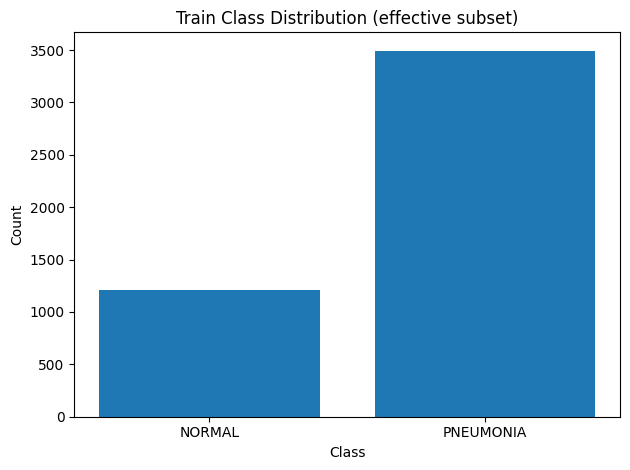
\includegraphics[width=0.7\linewidth]{DataDistribution.png}
    \caption{Class distribution in the training set.}
    \label{fig:train-class-distribution}
\end{figure}
Pneumonia cases are approximately three times more frequent than normal cases. To mitigate training bias from this class imbalance, we employ class weighting in the loss function, encouraging the model to learn balanced representations for both classes. The patients' have their personal information removed for the purposes of maintaining their privacy. The Operationalization of medical diagnoses is simple because the problem is very objective and requires the use of Experts to do the labeling. 


Together, these dataset preparation strategies provide a solid and clinically relevant foundation for building an automated pediatric pneumonia diagnosis system.



\section{Features}

% Describe any features you used for your model, or how your data was input to your model. Are you doing feature engineering or feature selection? Are you learning embeddings? Is it all part of one neural network? Refer to item 2. This may range from 0.25 pages to 0.5 pages.

Our model processes the input chest X-ray images by first applying augmentations and normalization to prepare the data for training. The images are originally grayscale but are converted into three-channel format to be compatible with the pretrained ResNet18 model we use. 
The network learns features automatically through fine-tuning the pretrained model. This means the model adjusts both low-level and higher-level layers to better capture patterns specific to pneumonia detection. We do not perform any manual feature engineering beyond the 
applied data augmentations. The representations are learned end-to-end, enabling the model to identify relevant structures and textures within the X-ray images that distinguish normal lungs from bacterial pneumonia.

\section{Implementation}

% Describe your model and implementation here. Refer to item 4. This may take around a page.


The model uses a ResNet18 convolutional neural network pretrained on ImageNet. Initially, we freeze all pretrained layers except the final fully connected layer, which is replaced to suit our binary pneumonia classification task. In this stage, only the classification head is trained, enabling the network to learn the mapping from extracted features to target labels while keeping the general feature extractor unchanged.
Once the classification head achieves satisfactory performance, we unfreeze the last convolutional block to fine-tune deeper layers. This process allows the network to adapt more task-specific features relevant to pediatric chest X-rays and pneumonia detection. We apply a reduced learning rate during fine-tuning to stabilize training and preserve useful pretrained representations.

To address class imbalance in the dataset, we use a weighted cross-entropy loss, formulated as:

\begin{equation}
\mathcal{L} = - \sum_{i=1}^N w_{y_i} \log p(y_i \mid \mathbf{x}_i)
\label{eq:weighted_cross_entropy}
\end{equation}

Here, \(N\) is the number of samples, \(y_i\) is the true label of sample \(i\), \(w_{y_i}\) is the corresponding class weight compensating for imbalance, and \(p(y_i \mid \mathbf{x}_i)\) is the predicted probability for the correct class given input \(\mathbf{x}_i\).

Training is performed using the Adam optimizer with weight decay to regularize model parameters and reduce overfitting. We utilize early stopping based on the validation F1-score to halt training when improvements plateau, ensuring the preservation of the best model weights.
For baseline comparison, a simple majority-class classifier is implemented, which always predicts the most frequent class in the training set. This baseline sets a minimal performance bar that our trained model is expected to exceed.
Data augmentation and preprocessing during training contribute to model robustness. Challenges encountered include tuning when to freeze or unfreeze layers and selecting appropriate learning rates, addressed through iterative experimentation guided by validation metrics.

The modular design of the implementation facilitates easy extension with alternative models, loss functions, or augmentation methods in future work. Overall, this transfer learning approach provides a strong framework for pediatric pneumonia classification with promising initial results.
\section{Results and Evaluation}

% How are you evaluating your model? What results do you have so far? What are your baselines? Refer to item 5. This may take around 0.5 pages.

We evaluate our model using stratified training, validation, and test splits.The validation set is used for hyperparameter tuning and early stopping, while the test set provides an unbiased estimate of final model performance.

Our evaluation metrics include accuracy, precision, recall, F1-score, and ROC-AUC. Accuracy measures the overall correct predictions; precision and recall focus on positive (pneumonia) detection performance, which is critical in a medical context to minimize missed diagnoses. 
The F1-score balances precision and recall, and the ROC-AUC quantifies the model’s discrimination ability across thresholds.

The baseline model used for comparison is a majority-class classifier that predicts the most frequent class in the training data.

We also compare against a majority-class baseline and visualize performance using a confusion matrix. The CNN substantially outperforms the baseline across all metrics, with F1-score improving from ~0.55 to >0.85 and recall notably higher, indicating fewer missed pneumonia cases.

We plan to incorporate k-fold cross-validation in future work for more robust performance estimates.
\begin{figure}[h]
    \centering
    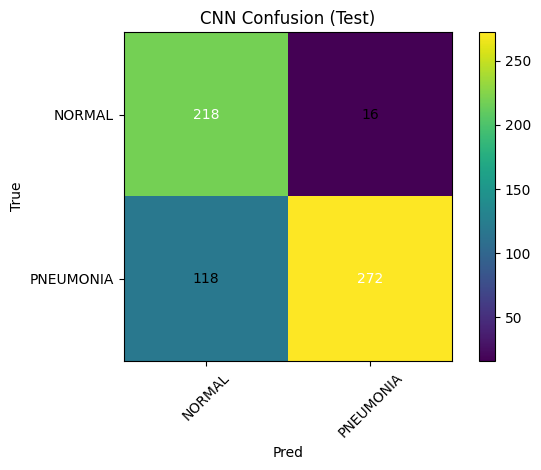
\includegraphics[width=0.7\linewidth]{ConfusionMatrix.png}
    \caption{Confusion matrix showing model performance on the test set.}
    \label{fig:confusion-matrix}
\end{figure}


Specifically, the validation F1-score improved from approximately 0.55 (baseline) to over 0.85 with the CNN. Recall increased notably, signaling fewer missed pneumonia cases. 
Confusion matrices further confirm enhanced true positive detection while controlling false positives.
These preliminary results demonstrate that fine-tuning the pretrained ResNet18 with our preprocessing and augmentation pipeline yields a robust pneumonia classifier with strong generalization to unseen data.
Future milestones include implementing k-fold cross-validation for more reliable estimates and further interpreting misclassification patterns to refine the model.




% Write about your plans for the remainder of the project. This should include a discussion of the feedback you received from your TA, and how you plan to improve your approach. Reflect on your implementation and areas for improvement. Refer to item 6. This may be around 0.5 pages.

\section{TA Feedback and Reflection}
The primary feedback from our TA emphasized the importance of using a simple baseline for comparison, specifically the majority-class classifier. This baseline predicts the most frequent class in the training data and establishes a clear performance threshold that the CNN model should surpass. Including such a baseline is essential for contextualizing model results and avoiding overstated performance claims.

Reflecting on this advice, we integrated the majority baseline into our evaluation framework and confirmed that our CNN model consistently outperforms it across key metrics. This strengthens confidence in the effectiveness of our transfer learning approach for pneumonia detection.

The TA also recommended focusing on binary classification between Normal and Bacterial Pneumonia instead of including Viral Pneumonia. This simplifies the task and keeps the project scope focused. All data preparation and model design follow this two-class goal, with the majority baseline serving as a clear reference point. A multiclass version may be explored later as an extension to this project.

In addition, the TA, mentioned that we could attempt to use multiple models (ie in a strategy similar to transfer learning), to use CNN features with an SVM which is a useful consideration we can make as we move forward

Overall, the TA’s guidance reinforced the importance of rigorous benchmarking and comparative evaluation, which will remain central to our approach in future milestones.

Our Plans moving forward are centered mostly around expanding on the strategies we've utilized so far to differentiate our implementation.
\section{Template Notes}

% You can remove this section or comment it out, as it only contains instructions for how to use this template. You may use subsections in your document as you find appropriate.

\subsection{Tables and figures}

See Table~\ref{citation-guide} for an example of a table and its caption.
See Figure~\ref{fig:experiments} for an example of a figure and its caption.


\begin{figure}[t]
  \includegraphics[width=\columnwidth]{example-image-golden}
  \caption{A figure with a caption that runs for more than one line.
    Example image is usually available through the \texttt{mwe} package
    without even mentioning it in the preamble.}
  \label{fig:experiments}
\end{figure}

\begin{figure*}[t]
  \includegraphics[width=0.48\linewidth]{example-image-a} \hfill
  \includegraphics[width=0.48\linewidth]{example-image-b}
  \caption {A minimal working example to demonstrate how to place
    two images side-by-side.}
\end{figure*}


\subsection{Citations}

\begin{table*}
  \centering
  \begin{tabular}{lll}
    \hline
    \textbf{Output}           & \textbf{natbib command} & \textbf{ACL only command} \\
    \hline
    \citep{Gusfield:97}       & \verb|\citep|           &                           \\
    \citealp{Gusfield:97}     & \verb|\citealp|         &                           \\
    \citet{Gusfield:97}       & \verb|\citet|           &                           \\
    \citeyearpar{Gusfield:97} & \verb|\citeyearpar|     &                           \\
    \citeposs{Gusfield:97}    &                         & \verb|\citeposs|          \\
    \hline
  \end{tabular}
  \caption{\label{citation-guide}
    Citation commands supported by the style file.
  }
\end{table*}

Table~\ref{citation-guide} shows the syntax supported by the style files.
We encourage you to use the natbib styles.
You can use the command \verb|\citet| (cite in text) to get ``author (year)'' citations, like this citation to a paper by \citet{Gusfield:97}.
You can use the command \verb|\citep| (cite in parentheses) to get ``(author, year)'' citations \citep{Gusfield:97}.
You can use the command \verb|\citealp| (alternative cite without parentheses) to get ``author, year'' citations, which is useful for using citations within parentheses (e.g. \citealp{Gusfield:97}).

\subsection{References}

\nocite{Ando2005,andrew2007scalable,rasooli-tetrault-2015}

Many websites where you can find academic papers also allow you to export a bib file for citation or bib formatted entry. Copy this into the \texttt{custom.bib} and you will be able to cite the paper in the \LaTeX{}. You can remove the example entries.

\subsection{Equations}

An example equation is shown below:
\begin{equation}
  \label{eq:example}
  A = \pi r^2
\end{equation}

Labels for equation numbers, sections, subsections, figures and tables
are all defined with the \verb|\label{label}| command and cross references
to them are made with the \verb|\ref{label}| command.
This an example cross-reference to Equation~\ref{eq:example}. You can also write equations inline, like this: $A=\pi r^2$.


% \section*{Limitations}

\section*{Team Contributions}

% Write in this section a few sentences describing the contributions of each team member. What did each member work on? Refer to item 7.
Luna worked on data preprocessing and augmentation, addressing class imbalance. Andrew focused on model adaptation, training, and hyperparameter tuning. Djordje handled evaluation, baselines, and visualization. All contributed equally to report writing and refinement.
% Bibliography entries for the entire Anthology, followed by custom entries
%\bibliography{custom,anthology-overleaf-1,anthology-overleaf-2}

% Custom bibliography entries only
\bibliography{custom}

% \appendix

% \section{Example Appendix}
% \label{sec:appendix}

% This is an appendix.

\end{document}
